\documentclass[12pt]{article}

% Packages
\usepackage{booktabs}   % for \toprule, \midrule, \bottomrule
\usepackage{geometry}   % optional: nicer margins
\geometry{margin=1in}
\usepackage{amsmath, amssymb}
\usepackage{setspace}
\usepackage{hyperref}
\usepackage{graphicx}
\onehalfspacing

\title{Pijoan-Mas (2006): Precautionary Savings\\or Working Longer Hours?}
\date{March 16, 2024}

\begin{document}
	
	\maketitle
	
	\section*{Model}
	
	Here I present a brief description of the model in Pijoan-Mas (2006). Households face the following problem:
	
	\begin{equation*}
		V(a, \varepsilon) = \max_{c, a', h} \left\{ \frac{c^{1 - \sigma}}{1 - \sigma} + \lambda \frac{(1 - h)^{1 - \nu}}{1 - \nu} + \beta \sum_{\varepsilon'} \Gamma_{\varepsilon, \varepsilon'} V(a', \varepsilon') \right\}
	\end{equation*}
	
	subject to
	
	\begin{equation*}
		c + a' = w \varepsilon h + (1 + r)a
	\end{equation*}
	
	\begin{equation*}
		c \geq 0, \quad 0 \leq h \leq 1, \quad a' \geq 0.
	\end{equation*}
	
	The individual state variables are asset holdings $a$ (endogenous) and the idiosyncratic shock $\varepsilon$ (exogenous, denoted $z$ in the toolkit notation). $\Gamma_{\varepsilon, \varepsilon'}$ denotes the transition matrix of the Markov chain over $\varepsilon$, with $\sum_{\varepsilon'} \Gamma_{\varepsilon, \varepsilon'} = 1$ for all $\varepsilon$.
	
	Households choose consumption $c$, hours of work $h$, and next-period assets $a'$. The policy functions are denoted as $c = g_c(a, \varepsilon)$, $h = g_h(a, \varepsilon)$, and $a' = g_a(a, \varepsilon)$.
	
	Factor prices $r$ and $w$ are pinned down by the first-order conditions of the representative firm:
	
	\begin{align*}
		r &= (1 - \theta) \left(\frac{K}{L}\right)^{-\theta} - \delta \\
		w &= \theta \left(\frac{K}{L}\right)^{1 - \theta}
	\end{align*}
	
	The aggregate production function is:
	
	\begin{equation*}
		Y = K^{1 - \theta} L^{\theta}
	\end{equation*}
	
	The market clearing conditions are:
	
	\begin{align*}
		K &= \int g_a(a, \varepsilon) \, d\mu(a, \varepsilon) \\
		L &= \int \varepsilon g_h(a, \varepsilon) \, d\mu(a, \varepsilon)
	\end{align*}
	
	where $\mu$ is the stationary distribution. Then, by Walras' Law, the aggregate resource constraint of the economy is automatically satisfied:
	
	\begin{equation*}
		C + \delta K = K^{1 - \theta} L^{\theta}
	\end{equation*}
	

\section*{Replication results}

	% Include the table file
	\begin{table}[!htbp]
\centering
\caption{Calibration targets and model parameters}
\begin{tabular}{llll}
\toprule
Parameter & Description & Target & Value \\
\midrule
$\sigma$  & Coeff. risk aversion   & corr(h,eps)= 0.019 & 1.456 \\
$\nu$     & Inverse elast. leisure & cv(h)= 0.207       & 2.800 \\
$\lambda$ & Weight of leisure      & H= 0.354           & 0.884 \\
$\beta$   & Discount factor        & K/Y= 2.998         & 0.945 \\
$\theta$  & Labor share            & wL/Y= 0.640        & 0.640 \\
$\delta$  & Capital depreciation   & I/Y= 0.249         & 0.083 \\
\bottomrule
\end{tabular}
\end{table}


	\begin{table}[!htbp]
\centering
\caption{Distributional statistics}
\begin{tabular}{llcccccc}
\toprule
Variable & $cv$ & Gini & $q_1$ & $q_2$ & $q_3$ & $q_4$ & $q_5$ \\
\midrule
\textbf{Hours} &   &  &   &  &  &  &  \\
Model $E_0$ & 0.20 & 0.11 & 0.24 & 0.34 & 0.37 & 0.39 & 0.42 \\
\addlinespace
\textbf{Earnings} &   &  &   &  &  &  &  \\
Model $E_0$ & 0.64 & 0.32 & 7.4 & 12.4 & 17.3 & 23.0 & 39.8 \\
\addlinespace
\textbf{Wealth} &   &  &   &  &  &  &  \\
Model $E_0$ & 1.36 & 0.64 & 0.1 & 2.3 & 9.4 & 23.3 & 64.9 \\
\bottomrule
\end{tabular}
\\[3ex]
\raggedright\footnotesize{\textit{Notes.} $cv$ refers to coefficient of variation. $q_1, \dots, q_5$ refer, for earnings and wealth, to the share held by all people in the corresponding quintile with respect to the total. However, for hours it is the average number of hours worked by people in the corresponding quintile.}\\
\normalsize
\end{table}

	
	\begin{figure}[!htbp]
		\centering
		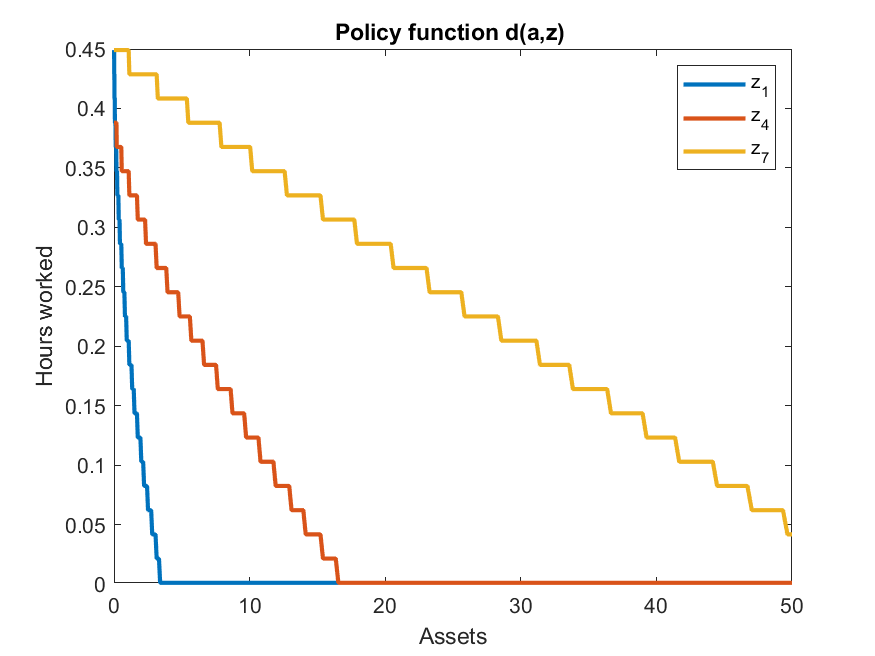
\includegraphics[width=0.7\textwidth]{pol_hours.png}
		\caption{Policy function for hours worked}
		\label{fig:pol_hours}
	\end{figure}

\begin{figure}[!htbp]
	\centering
	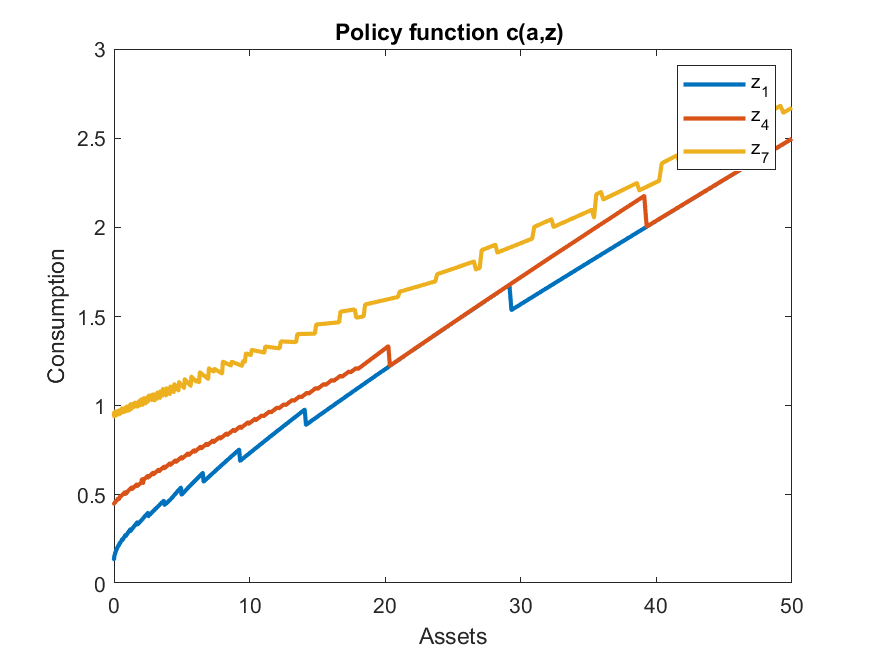
\includegraphics[width=0.7\textwidth]{pol_cons.png}
	\caption{Policy function for consumption}
	\label{fig:pol_hours}
\end{figure}
	
	\section*{References}
	
	Pijoan-Mas, Josep, ``Precautionary Savings or Working Longer Hours?,'' \emph{Review of Economic Dynamics}, April 2006, 9(2), 326--352.
	
\end{document}
